\documentclass[tikz, border=10pt]{standalone}
\usetikzlibrary{shapes.geometric, arrows, positioning, fit, calc, backgrounds}

\begin{document}

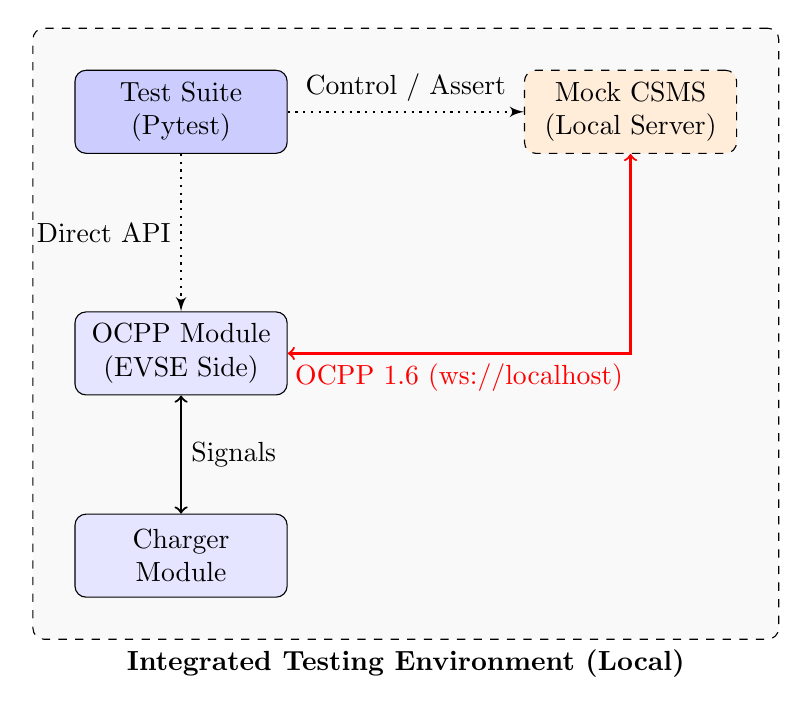
\begin{tikzpicture}[
    node distance=2.5cm,
    block/.style={rectangle, draw, fill=blue!10, text width=7em, text centered, rounded corners, minimum height=3em},
    mock/.style={rectangle, draw, fill=orange!15, text width=7em, text centered, rounded corners, minimum height=3em, dashed},
    container/.style={draw, rectangle, dashed, inner sep=1.5em, fill=gray!5, rounded corners},
    line/.style={draw, -latex', thick},
    api/.style={draw, -latex', thick, dashed, color=blue},
    ocpp/.style={draw, -latex', thick, color=red},
    control/.style={draw, -latex', thick, dotted, color=black}
]

    % Test Automation
    \node [block, fill=blue!20] (testsuite) {Test Suite (Pytest)};
    
    % Mock CSMS (Local)
    \node [mock, right=3cm of testsuite] (mock_csms) {Mock CSMS\\(Local Server)};
    
    % EVSE System
    \node [block, below=2cm of testsuite] (interface) {OCPP Module\\(EVSE Side)};
    \node [block, below=1.5cm of interface] (charger) {Charger Module};
    
    % Group Containers
    \begin{scope}[on background layer]
        \node [container, fit=(testsuite) (mock_csms) (interface) (charger)] (local_env) {};
    \end{scope}

    \node [below] at (local_env.south) {\textbf{Integrated Testing Environment (Local)}};

    % Connections
    
    % Test Control Flow
    \path [control] (testsuite) -- node [midway, above] {Control / Assert} (mock_csms);
    \path [control] (testsuite) -- node [midway, left] {Direct API} (interface);
    
    % OCPP Connection (Local Loopback)
    \path [ocpp, <->] (interface) -| node [near start,below] {OCPP 1.6 (ws://localhost)} (mock_csms);
    
    % Internal EVSE State 
    \path [line, <->] (interface) -- node [midway, right] {Signals} (charger);

\end{tikzpicture}

\end{document}
